%%%%%%%%%%%%%%%%%%%%%%%%%%%%%%%%%%%%%%%%%%%%%%%%%%%%%%%%%%%%%%%%%%%%%%
%
% 都市システム工学科 特別研究概要テンプレート(2013 年度版)
%
%%%%%%%%%%%%%%%%%%%%%%%%%%%%%%%%%%%%%%%%%%%%%%%%%%%%%%%%%%%%%%%%%%%%%%

\documentclass[a4paper,10pt]{jarticle}
\usepackage[dvips]{graphicx}
\usepackage{amsmath}
\usepackage{setspace}
\usepackage{ascmac}

\textwidth      18.0cm
\textheight     27.0cm
\oddsidemargin  -1.0cm
\evensidemargin -1.0cm
\topmargin      -2.3cm
\footskip        0.5cm
\columnsep       2.5zw

\renewcommand{\baselinestretch}{0.95}
\pagestyle{empty}

\makeatletter
\def\section{\@startsection {section}{1}{\z@}{-3.5ex plus -1ex minus 
 -.2ex}{2.3ex plus .2ex}{\normalsize \bf}}
\def\subsection{\@startsection {subsection}{1}{\z@}{-3.5ex plus -1ex minus 
 -.2ex}{2.3ex plus .2ex}{\normalsize \bf}}
\makeatother

\begin{document}
\twocolumn[
\begin{center}
 \vspace{-2mm}
 \begin{large}
  {\bf 最大の移動時間を最小化する教室割当問題の定式化と求解}\\
 \end{large}
 \vspace{-2mm}
\end{center}
 {\bf システムモデリング研究室}
 \hfill {\bf 都 11-23 岡崎 俊介}
 \vspace{5mm}
] % End of twocolumn

%% vspace のあとの寸法は,出来上がりイメージを見て適宜修正すること

%%%%%%%%%%%%%%%%%%%%%%%%%%%%%%%%%%%%%%%%%%%%%%%%%%%%%%%%%%%%%%%%%%%%%%
\vspace{-8mm}
\section{はじめに}
\vspace{-2.5mm}
%%%%%%%%%%%%%%%%%%%%%%%%%%%%%%%%%%%%%%%%%%%%%%%%%%%%%%%%%%%%%%%%%%%%%%

 一般に,大学の授業においては,それを開講する教室を割り当てる必要がある.
この問題を本研究では教室割当問題と呼ぶことにする.
現在,関西大学においては,授業に対する教室の割当は全て手動で行われている.

教室割当の自動化については,例えば,マルチエージェントシミュレーションを行い,学生の移動時間を最小化した教室配置を行う研究がある\cite{教室割当問題2}.
これに対し本研究では,教室割当問題を最適化問題として定式化し,最適化ソルバーを用いてそれを解くことを試みる.

実は\cite{先行研究}でも同じような研究が行われており,学生の移動時間の総和を最小化するような教室割当を求めることを目標とした最適化問題を解いている.
しかしながら,最適解を求めることができないケースが多く見られた.

そこで本研究では,\cite{先行研究}とは目的を変更し,学生の移動時間の最大値を最小にするような教室割当を求めることを目指す.

%%%%%%%%%%%%%%%%%%%%%%%%%%%%%%%%%%%%%%%%%%%%%%%%%%%%%%%%%%%%%%%%%%%%%%
\vspace{-4mm}
\section{先行研究の問題点と本研究でのアプローチ}
\vspace{-2.5mm}
%%%%%%%%%%%%%%%%%%%%%%%%%%%%%%%%%%%%%%%%%%%%%%%%%%%%%%%%%%%%%%%%%%%%%%
%%%%%%%%%%%%%%%%%%%%%%%%%%%%%%%%%%%%%%%%%%%%%%%%%%%%%%%%%%%%%%%%%%%%%%
%\subsection{・・・}
%\vspace{-2mm}
%%%%%%%%%%%%%%%%%%%%%%%%%%%%%%%%%%%%%%%%%%%%%%%%%%%%%%%%%%%%%%%%%%%%%%
 前節でも述べたように,先行研究\cite{先行研究}では最適解を求めることができないケースが多く見られた.
その理由を検証した結果,
\vspace{-2mm}
\begin{itemize}
\setlength{\parskip}{1mm} % 段落間
\setlength{\itemsep}{0mm} % 項目間
\item 制約条件の定式化に誤りがある
\item 変数が多く,最適化計算に時間がかかってしまう
\end{itemize}
\vspace{-2mm}
ということがわかった.
また,\cite{先行研究}での目的関数は全学生の移動時間の総和を最小化する教室割当を求めようとしているが,これによって目的関数が複雑になっていることもわかった.

そこで本研究では,先行研究での誤りを修正するとともに,各授業の開講曜限が定められているとき,
各休み時間における\underline{学生の最大の移動時間を最小化する}ような教室の割当を求めることを目的とする.

\if0
%%%%%%%%%%%%%%%%%%%%%%%%%%%%%%%%%%%%%%%%%%%%%%%%%%%%%%%%%%%%%%%%%%%%%%
\vspace{-4mm}
\subsection{方法}
\vspace{-2.5mm}
%%%%%%%%%%%%%%%%%%%%%%%%%%%%%%%%%%%%%%%%%%%%%%%%%%%%%%%%%%%%%%%%%%%%%%
\fi
本研究では,この問題の最適解を求めるためのアプローチとして,最適化問題の中に移動時間の上限を定めるパラメータを準備する.
そして,そのパラメータを調整しながら問題を解き,実行可能解が得られるパラメータの最小値を求める.
これが最大の移動時間の最小値となる.

\vspace{-3.0mm}
\section{定式化の概要}
\vspace{-2.0mm}
 本研究で解く最適化問題は,以下のような制約条件と目的関数を持つ.
\vspace{-1.5mm}
\begin{itemize}
\setlength{\parskip}{0.5mm} % 段落間
\setlength{\itemsep}{0mm} % 項目間
\item{ [絶対制約1] : 1つの曜限において各教室には2つ以上の授業を割り当てられない.}
\item { [絶対制約2] : 各授業には必ず1つの教室を割り当てなければならない.}
\item { [絶対制約3] : 受講人数が教室の定員を超えて教室に授業を割り当ててはならない.}
\item { [絶対制約4-1] : 特定の授業は指定された教室で開講されなければならない.}
\vspace{-1.5mm}
\begin{itemize}
\item 特定の設備を必要とする授業に,その設備が整っている,指定された教室を割り当てるための制約である.
\end{itemize}
\vspace{-1.5mm}
\item { [絶対制約4-2] : 指定された授業でないものは特殊教室で開講されてはいけない.}
\vspace{-1.5mm}
\begin{itemize}
\item 一般的な授業に特殊教室を割り当てることを避けるための制約である.
\end{itemize}
\vspace{-1.5mm}
\item { [絶対制約5] : 移動時間は指定した時間以内でなければならない.}
\vspace{-1.5mm}
\begin{itemize}
\item 休み時間を授業の準備に費やせるように,移動時間を制限するための制約である.
\end{itemize}
\vspace{-1.5mm}
\item { [絶対制約6] : 特別連続授業は同じ教室で開講されなければならない.}
\vspace{-1.5mm}
\begin{itemize}
\item 特別連続授業(授業内容が同一,または非常に関連性の高い2限以上連続で開講される授業)を同一教室で行うための制約である.
\end{itemize}
\vspace{-1.5mm}
\item { [考慮制約1] : 教室内の人が入れ替わる際の混雑ができるだけ発生しないほうが好ましい.}
\item { [考慮制約2] : 希望教室があれば,その教室で授業を開講したい.}
\vspace{-1.5mm}
\begin{itemize}
\item できるだけ学生や教員が希望した教室で授業を開講するための制約である.
\end{itemize}
\vspace{-1.5mm}
\item {[目的関数]: 考慮制約1を満たせていない場合に発生する違反指標の合計と,考慮制約2を満たせた場合の指標の合計に,
それぞれ重みを乗じたものの合計値を最小化するように定める.
ただし,考慮制約2の指標については,制約を満たした場合に指標が発生するので,重みは負の値にしなければならない.}
\end{itemize}

\vspace{-2.0mm}

%%%%%%%%%%%%%%%%%%%%%%%%%%%%%%
\vspace{-4mm}
\section{数値実験}
\vspace{-2.5mm} 
%%%%%%%%%%%%%%%%%%%%%%%%%%%%%%
 本研究で用いた計算環境を表\ref{kankyo1}に示す.
\vspace{-5.0mm}
\vspace{-1.5mm}
\begin{table}[htb]
\begin{center}
\caption{計算環境}
\vspace{-5mm} 
\label{kankyo1}
\scalebox{0.9}[0.9]{ 
\begin{tabular}{c|c}
\hline
OS & Microsoft Windows 7 Home Premium Service Pack 1\\
CPU &Intel(R) Core(TM) i5-2520M CPU @ 2.50GHz\\ 
メモリ & 8.0 GB\\
ソルバー&IBM ILOG CPLEX 12.4.0.0\\
\hline
\end{tabular}
}
\end{center}
\end{table}
\vspace{-5.0mm}
\vspace{-2.0mm}

また,計算には以下のようなデータを用いた.
\vspace{-3.0mm}
\begin{itemize}
\setlength{\parskip}{0cm} % 段落間
\setlength{\itemsep}{0cm} % 項目間
\item 使用教室\\
第4学舎にある一般教室である44教室,及びOD教室などの特殊教室である23教室の,合計67教室を対象としている.
\item 対象授業\\
理工系学部で開講される全授業を対象としている.
\end{itemize}

\vspace{-7.0mm}
\subsection{予備実験}
\vspace{-3.0mm}
 本研究では,本実験の方針を定めるために,以下の予備実験を行った.
\vspace{-2.0mm}
\begin{itemize}
\setlength{\parskip}{0cm} % 段落間
\setlength{\itemsep}{0cm} % 項目間
\item 予備実験1:サンプルデータを用いた数値実験
\vspace{-1.5mm}
\begin{itemize}
\item サンプルデータを用いて定式化したモデルが意図した挙動を示すかどうかを確認する
\end{itemize}
\vspace{-1.5mm}
\item 予備実験2:春学期火曜午前の実データを用いた数値計算
\vspace{-1.5mm}
\begin{itemize}
\item 実データが正しく準備されているかの確認と,最適解が得られるまでに要する時間の確認を行う
\end{itemize}
\vspace{-1.5mm}
\end{itemize}
\vspace{-1.5mm}

予備実験1で得られた解を確認すると,全ての絶対制約が満たされており,各考慮制約も正しく動作をしていた.
また,予備実験2では数秒で解を得ることができ,得られた解を確認すると,実際の規模の問題に対しても正しく動作をしていたことがわかった.
\vspace{-4.0mm}

\subsection{本実験}
\vspace{-3.0mm}
 本研究では,以下の実験を行った.\\
\vspace{-4mm}
\vspace{-3.0mm}
\begin{itemize}
\setlength{\parskip}{1mm} % 段落間
\setlength{\itemsep}{1mm} % 項目間
\item 本実験1:最大移動時間の最小値を求める実験
\begin{itemize}
\vspace{-1.5mm}
\item 実データ(春学期・秋学期,月曜~土曜,午前・午後で分けて作成した24通りのデータ)を用いて,最適解を求める.
\end{itemize}
\vspace{-1.5mm}
\item 本実験2:本実験1の結果,最大移動時間が極端に大きくなる授業を取り除いて行う実験
\begin{itemize}
\vspace{-1.5mm}
\item 本実験1において最大移動時間が他の曜限と比べて極端に大きい春学期月曜午後,及び春学期木曜午後のデータから,最も移動時間を要していた授業を取り除いた場合の最適解を求める.
\end{itemize}
\vspace{-1.5mm}
\item 本実験3:希望教室を設定した春学期火曜午前のデータを用いた実験
\vspace{-1.5mm}
\begin{itemize}
\item 春学期火曜午前のデータにおける1限に開講される3つの授業に,それぞれ同じ教室を2つずつ用意して最適解を求める.
\end{itemize}
\vspace{-1.5mm}
\end{itemize}
\vspace{-2.0mm}
%\vspace{-1.5mm}

実験1の結果,全ての曜限において解を求めることができた.
また,計算時間はいずれも100秒以内であった.
\vspace{-7.0mm}
\begin{table}[h]
\vspace{-2.0mm}
\begin{center}
\caption{本実験1の実験結果(秒)}
\label{jikken1}
\scalebox{1.0}[1.0]{ 
\begin{tabular}{l|cc|cc}
\hline
曜日 & \multicolumn{2}{c|}{春学期} & \multicolumn{2}{|c}{秋学期}\\
\hline
 & 最大 & 平均 &  最大 & 平均\\
\hline
月曜午前  & 96  & 58.3 & 50  & 22.4\\
  午後  & 251 & 53.6 & 67  & 27.3\\
火曜午前  & 76  & 39.4 & 68  & 32.9\\
  午後  & 141 & 53.8 & 49  & 12.5\\
水曜午前  & 58  & 28.4 & 57  & 30.2\\
  午後  & 52  & 18.0 & 123 & 43.1\\
木曜午前  & 34  & 14.1 & 58  & 39.4\\
  午後  & 251 & 37.3 & 60  & 21.7\\
金曜午前  & 103 & 47.5 & 89  & 45.9\\
  午後  & 74  & 20.9 & 80  & 28.4\\
土曜午前  & 33  & 12.6 & 34  & 19.7\\
  午後  & 27  & 7.3 & 74  & 52.7\\
\hline
\end{tabular}
}
\end{center}
\end{table}
\vspace{-5.0mm}

表\ref{jikken1}は本実験1で求めた最小化された移動時間の最大と平均を示している.
また,図\ref{omo12}は,移動時間(5秒ごと)制の学生数を表している.
これより,学生の一部は移動時間が大きいが,全体的には移動時間がある程度短くなるような教室割当が求められていることがわかる.


\begin{table}[h]
\vspace{-2.0mm}
\begin{center}
\caption{本研究と先行研究の比較(春学期月曜午後)}
\label{hikaku2}
\begin{tabular}{r|cc}
\hline
&本研究&先行研究 \\
\hline
移動時間(秒)& 96  & 最適解求解不可  \\  
制約数& 2569 &  933306 \\ 
変数の数&1854 & 4781 \\
計算時間(秒) &4.34&  3600\\
\hline
\end{tabular}
\vspace{-7.0mm}
\end{center}
\end{table}


\if0
\begin{table}[h]
\caption{本実験1の結果}
\label{hikaku1}
\begin{center}
\begin{tabular}{|r|ccccc|}
\hline
&移動時間&制約数&変数の数&計算時間\\
\hline
本研究 & 96  & 2569 & 1854 &  4.34\\  
先行研究 & 解なし & 933306 & 4781 &  3600\\ 
\hline
\end{tabular}
\end{center}
\end{table}
\fi

また,表\ref{hikaku2}により,本研究で提案した手法では,先行研究よりも制約数,及び変数の数を大きく削減できていることがわかる.
これは,全ての曜限において共通していた.
このことより,期待した実験結果を得ているといえる.

表\ref{jikken2}は本実験2の結果である.
表\ref{jikken2}より,これは本実験1におけるその他の曜限の結果に近い結果であり,特定の授業だけが移動に時間を要していたということが確認できた.
%また,平均移動時間も減少してる
この結果より,移動時間が大きくなりそうな授業の教室割当をあらかじめ決めておき,その後に提案手法により残りの授業の教室割当を決めれば,よい割当が求められることがわかる.
\begin{figure}[thpb]
 \begin{center}
 \hspace{5mm} 
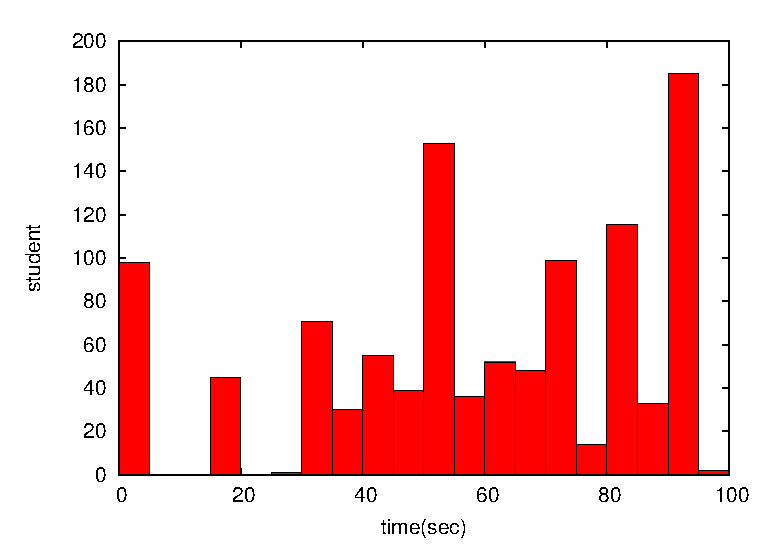
\includegraphics[bb=0 0 390 248,clip,scale=0.6]{oMo12_hist.eps}
 \hspace{-10mm} 
\vspace{-5mm}
  \caption{移動時間ごとの学生数(春学期月曜午前)}
  \label{omo12}
 \end{center}
\end{figure}
\vspace{-5mm}

\vspace{-3mm}
\begin{table}[h]
\vspace{-2.0mm}
\begin{center}
\caption{本実験2の実験結果}
\label{jikken2}
\begin{tabular}{c|cc}
\hline
曜日&最大&平均 \\
\hline
春学期月曜午後& 67 & 37.9  \\  
春学期木曜午後& 51 & 15.4 \\ 
\hline
\end{tabular}
\vspace{-5.0mm}
\end{center}
\end{table}


さらに,本実験3の結果,最大の移動時間の最小値は,希望を定めていない本実験1と同じ,76秒となった.
また,目的関数の値を確認すると,希望教室を最大限叶えることができていることがわかった.
この結果より,事前に希望を調べておき,それをできるだけ叶えるような教室割当が求められることがわかった.

%%%%%%%%%%%%%%%%%%%%%%%%%%%%%%%%%%%%%%%%%%%%%%%%%%%%%%%%%%%%%%%%%%%%%%
\vspace{-4mm}
\if0
\section{考察}
\vspace{-2.5mm}
%%%%%%%%%%%%%%%%%%%%%%%%%%%%%%%%%%%%%%%%%%%%%%%%%%%%%%%%%%%%%%%%%%%%%%
 本研究では,最大の移動時間を最小化するという方法をとることで,移動時間を最小化することができた.
これは,全ての制約式が正しく作動し,また制約や変数の数も先行研究より大きく削減できたことによって,計算範囲をうまく狭めることができたためではないかと考えられる.
また,本研究では最適解を求めるために何回も計算を行う必要があるが,全ての計算が100秒以内に終わっているので,回数を重ねても時間がかかってしまうことはない.
これは,実用性のある教室割当問題を解くことができているといえる.
また,実験2では,移動時間のかかってしまう授業を見つけ,また対処することもできた.
従って,本研究では融通のきく時間割作成を行うことが可能であるといえる.

%%%%%%%%%%%%%%%%%%%%%%%%%%%%%%%%%%%%%%%%%%%%%%%%%%%%%%%%%%%%%%%%%%%%%%
\vspace{-4mm}
\fi

\section{おわりに}
\vspace{-2.5mm}
%%%%%%%%%%%%%%%%%%%%%%%%%%%%%%%%%%%%%%%%%%%%%%%%%%%%%%%%%%%%%%%%%%%%%%

 本研究では,先行研究の誤りを正し,また異なる視点から教室割当問題を定式化し,それを最適化ソルバーで解くことで,最大の移動時間を最小化するような教室割当を求めることができた.

今後の課題として,本研究における教室割当を求める際に有用なインターフェイスを開発することが挙げられる.

\if0
文献や式・図表の引用は以下のように:
\begin{itemize}
 \item \cite{都市12}
 \item 式 (\ref{eq:G})
 \item 図 \ref{fig:1}
 \item 表 \ref{tb:1}
\end{itemize}
\fi
%%%%%%%%%%%%%%%%%%%%%%%%%%%%%%%%%%%%%%%%%%%%%%%%%%%%%%%%%%%%%%%%%%%%%%
\vspace{-2.5mm}
\begin{thebibliography}{9}
\vspace{-2.5mm}
%
%\bibitem{ハンドブック}
%久保幹雄,田村明久,松井知己 編集,応用数理計画ハンドブック,朝倉書店 (2002).

\vspace{-1.5mm}

\bibitem{先行研究}
鈴木健太,移動時間を最小化する教室割当問題の定式化と求解,関西大学環境都市工学部平成25年度卒業論文 (2014).
\vspace{-2.5mm}

\bibitem{教室割当問題2}
前川廣太郎,教室間移動時間最適化を目的としたマルチエージェントシミュレーションとGAの統合\\
http://nobuharaken.com/study/1705.html\\(2015年2月3日確認).

\end{thebibliography}
%%%%%%%%%%%%%%%%%%%%%%%%%%%%%%%%%%%%%%%%%%%%%%%%%%%%%%%%%%%%%%%%%%%%%%
\if0
\begin{figure}[htpb]
 \begin{center}
  
\includegraphics[scale=0.3]{./KU.eps}
  \caption{図や写真等のタイトルは下に配置}
  \label{fig:1}
 \end{center}
\end{figure}
 数式は,\verb|align| 環境を用いて入力すること.
%
\begin{align}
 G &= \sum_{n = 0}^\infty b_n(t)
 \label{eq:G} \\
 F &= \int_\Gamma \sin z \; {\rm d}z
 \label{eq:F}
\end{align}
%
\begin{table}
 \begin{center}
  \caption{表のタイトルは上に配置}
  \begin{tabular}{|l|l|l|}
   \hline
   A \hspace{2cm} & B \hspace{2cm} & C \hspace{2cm} \\
   \hline
   あ & い & う \\
   \hline
  \end{tabular}
  \label{tb:1}
 \end{center}
\end{table}
\fi

\end{document}

%%%%% End of file %%%%%

